% !TEX encoding = utf8
% !TEX program = xelatex

\documentclass[red,compress]{beamer}
\usetheme{Warsaw}

%\usepackage[noindent]{ctex}
\usepackage{fontspec,xunicode,xltxtra}
\usepackage{color}
\usepackage{amsmath}
\usepackage{graphicx}
\usepackage{wrapfig}
\usepackage{enumerate}


\graphicspath{ {./images/} }

\setmainfont{微软雅黑}
\setmonofont{微软雅黑}
\setsansfont{微软雅黑}
\XeTeXlinebreaklocale "zh"
\XeTeXlinebreakskip = 0pt plus 1pt

% 设置beamer 中公式字体
\usefonttheme{professionalfonts}
% 设置中文字体
%\setCJKmainfont[BoldFont={黑体}.ItalicFont={楷体}]{新宋体}

\begin{document}


\title{插值\&曲线拟合}
\author{YI Xinglu}
\date{\today}
\frame{\titlepage}
%---------------------
\begin{frame}
\frametitle{应用}
\begin{figure}
%\centering
	
\includegraphics[width=.4\linewidth]{quanhuang.png}
\end{figure}
\begin{figure}
	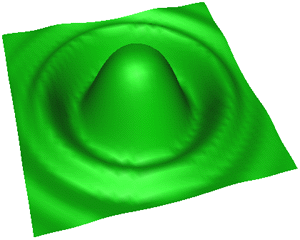
\includegraphics[width=.4\linewidth]{weightinterp2.png}
	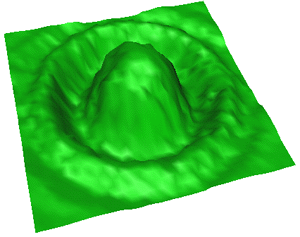
\includegraphics[width=.4\linewidth]{weightinterp6.png}
\end{figure}
\end{frame}
%---------------------
\begin{frame}
\frametitle{区别}
\begin{figure}
\centering
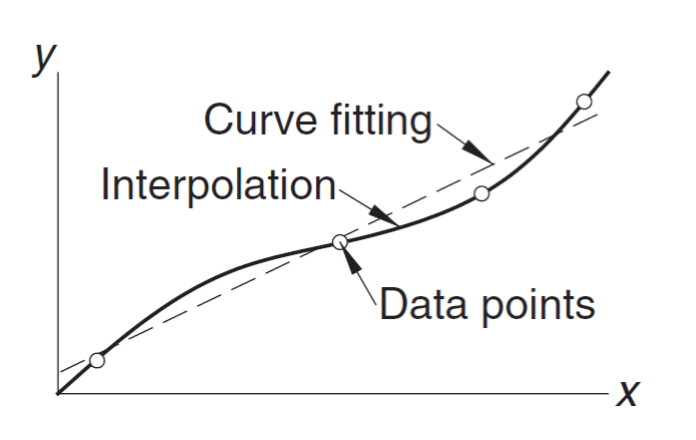
\includegraphics[width=0.75\textwidth]{int.png}
\end{figure}
\end{frame}
%---------------------
\begin{frame}
\frametitle{多项式插值}
\begin{itemize}
\item 拉格朗日插值(Lagrange)
\item 牛顿插值(Newton)
\item 三次样条插值(Cubic spline)
\item 曲线拟合(curve fitting)
\end{itemize}
\end{frame}
%---------------------
\begin{frame}
\frametitle{插值问题}
给定数据点列$(x_i,y_i), i=1,2,...,m$满足$x_1<x_2<\cdots<x_m$确定了一个函数$f:\mathbb{R}\rightarrow\mathbb{R}$使得
\begin{equation*}
	f(x_i)=y_i, i=1,2,...,m
\end{equation*}
$f$即为给定点列的插值函数.
\end{frame}
%---------------------
\begin{frame}
\frametitle{拉格朗日插值}
插值基函数
\begin{equation*}
	P_{n-1}(x)=\sum_{i=1}^{n}y_{i}l_{i}(x)
\end{equation*}
\begin{align*}
	l_{i}(x)&=\frac{x-x_1}{x_i-x_1}\cdot\frac{x-x_2}{x_i-x_2}\cdots\frac{x-x_{i-1}}{x_i-x_{i-1}}\cdot\frac{x-x_{i+1}}{x_i-x_{i+1}}\cdots\frac{x-x_n}{x_i-x_n} \\
	&=\prod_{\substack{j=1 \\ j\neq i}}^{n}\frac{x-x_j}{x_i-x_j}, i=1,2,...,n
\end{align*}
\end{frame}
%---------------------
\begin{frame}
\frametitle{拉格朗日插值}

\begin{columns}[T]
\column{0.6\textwidth}
对点列$(x_1,y_1),\cdots,(x_n,y_n)$,基函数$l_i(x)$是$n-1$阶多项式且有以下性质:
\begin{equation*}
\delta_{ij} = l_i(x_j)=
	\begin{cases}
        0 & \text{if $i\neq j$}\\
        1 & \text{if $i=j$}
    \end{cases}
\end{equation*}

\column{0.4\textwidth}
\begin{figure}
\center
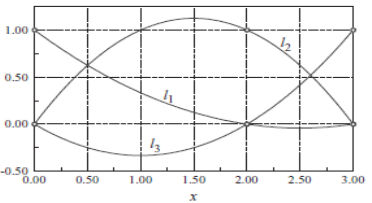
\includegraphics[width=\textwidth]{lagrange.png}
\end{figure}
\end{columns}

进而
\begin{equation*}
	P_{n-1}(x_j)=\sum_{i=1}^{n}y_{i}l_i(x_j)=\sum_{i=1}^{n}y_i\delta_{ij}=y_j
\end{equation*}

\end{frame}
%---------------------
\begin{frame}
\frametitle{秦九韶算法(1247)}

\begin{align*}
	p(x)&=\sum_{i=0}^{n}a_{i}x^i=a_0+a_1x+a_2x^2+\cdots+a_nx^n \\
	    &=a_0+x(a_1+x(a_2+\cdots+x(a_{n-1}+a_nx)\cdots))
\end{align*}

当$x=3$时,求值$f(x)=2x^3-6x^2+2x-1$
\begin{columns}[T]
\column{0.5\textwidth}
\begin{equation*}
\begin{array}{r|*{4}r}
	x_0 & x^3 & x^2 & x^1 & x^0 \\
	3   & 2   & -6  & 2   & -1  \\
	    &     & 6   & 0   & 6   \\
     \hline
	    & 2 & 0 & 2& 5
\end{array}
\end{equation*}

\column{0.5\textwidth}
\begin{figure}
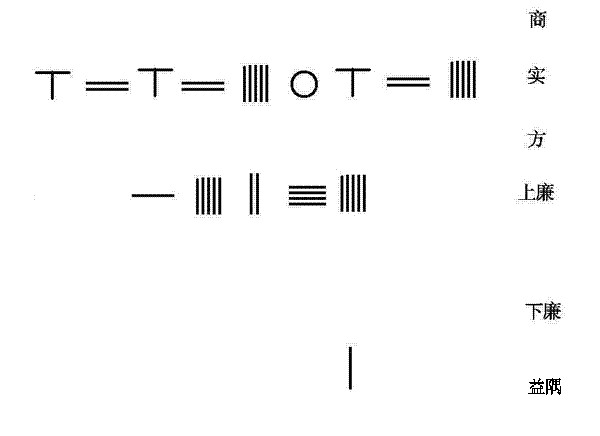
\includegraphics[width=0.7\textwidth]{qinjiushao.jpg}
\end{figure}
\end{columns}
\end{frame}
%---------------------

\begin{frame}
\frametitle{秦九韶算法(1247)}
\begin{itemize}
\item 使用单项形式求解$n$阶多项式的值需要至多$n$次加法和$\frac{n^2+n}{2}$次乘法
\item 秦九韶算法只需$n$次加法和$n$次乘法
\item 西方称此算法为霍纳(Horner--\textcolor{red}{1819})算法
\end{itemize}
\end{frame}
%---------------------
\begin{frame}
\frametitle{牛顿插值}
尽管Lagrange插值算法概念简单,但运算效率不高

\begin{align*}
	P_{n-1}(x)=a_1+(x-x_1)a_2+(x-x_1)(x-x_2)a_3+\cdots \\
		+(x-x_1)(x-x_2)\cdots(x-x_{n-1})a_n
\end{align*}
\begin{align*}
	P_2(x)&=a_1+(x-x_1)a_2+(x-x_1)(x-x_2)a_3\\
			&=a_1+(x-x_1)(a_2+(x-x_2)a_3)
\end{align*}

\end{frame}
%---------------------

\begin{frame}
\frametitle{牛顿插值}
由插值性得:$y_i=P_{n-1}(x_i),i=1,2,...,n.$即
\begin{flalign*}
	y_1&=a_1 &\\
	y_2&=a_1+(x_2-x_1)a_2 &\\
	\vdots &\\
	y_n&=a_1+(x_n-x_1)a_2+\cdots+(x_n-x_1)(x_n-x_2)\cdots(x_n-x_{n-1})a_n &
\end{flalign*}

\end{frame}
%---------------------

\begin{frame}
\frametitle{差商(Divided Differences)}

\begin{flalign*}
	\nabla y_i&=\frac{y_i-y_1}{x_i-x_1}, i=2,3,...,n &\\
	\nabla^2 y_i&=\frac{\nabla y_i-\nabla y_2}{x_i-x_2}, i=3,4,...,n &\\
	\nabla^3 y_i&=\frac{\nabla^2 y_i - \nabla^2 y_3}{x_i-x_3}, i=4,5,...,n &\\
	\vdots &\\
	\nabla^n y_n&=\frac{\nabla^{n-1} y_n - \nabla^{n-1} y_{n-1}}{x_n-x_{n-1}} &
\end{flalign*}

\end{frame}
%---------------------

\begin{frame}
\frametitle{牛顿插值}

\begin{equation*}
	a_1=y_1, \quad a_2=\nabla y_2, \quad a_3=\nabla^2y_3 \quad \cdots \quad a_n=\nabla^ny_n
\end{equation*}
\begin{equation*}
\begin{array}{c|*{5}c}
\hline
x_1 & y_1 & 	       &              &              & \\
x_2 & y_2 & \nabla y_2 &              &              & \\
x_3 & y_3 & \nabla y_3 & \nabla^2 y_3 &              & \\
x_4 & y_4 & \nabla y_4 & \nabla^2 y_4 & \nabla^3 y_4 & \\
x_5 & y_5 & \nabla y_5 & \nabla^2 y_5 & \nabla^3 y_5 & \nabla^4 y_5 \\
\hline 
\end{array}
\end{equation*}

\end{frame}
%---------------------

\begin{frame}
\frametitle{Neville算法}
\begin{itemize}
\item
牛顿插值可以重复计算插值点的值,如果只需计算一个插值点的值,Neville算法是更好的选择。

\item
$P_{i,j}$表示经过数据点$(x_k,y_k),k=i,i+1,\cdots,j$的$j-i$阶多项式,满足:
\begin{align*}
	P_{i,i}(x) &= y_i, \\
	P_{i,j}(x) &= \frac{(x_j-x)P_{i,j-1}(x)+(x-x_i)P_{i+1,j}(x)}{x_j-x_i}
\end{align*}

容易验证:$P_{i,j}(x_i)=y_i,\: P_{i,j}(x_j)=y_j$
\end{itemize}
\end{frame}
%---------------------

\begin{frame}
\frametitle{Neville算法}
\begin{equation*}
\begin{array}{r|*{5}c}
x_0 & P_{0,0}(x)=y_0 &            &            &            & \\
    &                & P_{0,1}(x) &            &            & \\
x_1 & P_{1,1}(x)=y_1 &            & P_{0,2}(x) &            & \\
    &                & P_{1,2}(x) &            & P_{0,3}(x) & \\
x_2 & P_{2,2}(x)=y_2 &            & P_{1,3}(x) &            & P_{0,4}(x) \\
    &                & P_{2,3}(x) &            & P_{1,4}(x) & \\
x_3 & P_{3,3}(x)=y_3 &            & P_{2,4}(x) &            & \\
    &                & P_{3,4}(x) &            &            & \\
x_4 & P_{4,4}(x)=y_4 &            &            &            &
\end{array}
\end{equation*}
\begin{equation*}
P_{0,4}(x)=\sum_{i=0}^{4}y_il_i(x)
\end{equation*}
\end{frame}
%---------------------

\begin{frame}
\frametitle{多项式插值的局限}
\begin{columns}[T]
\column{0.7\textwidth}
\begin{itemize}
\item 多项式插值的灵活性不好,数据点改变即需重新计算插值函数
\item 离关注点较远的数据点对插值的准确性没有太多贡献
\item 高阶多项式有在数据点之间会出现震荡
\end{itemize}

\column{0.3\textwidth}
\begin{figure}
\center
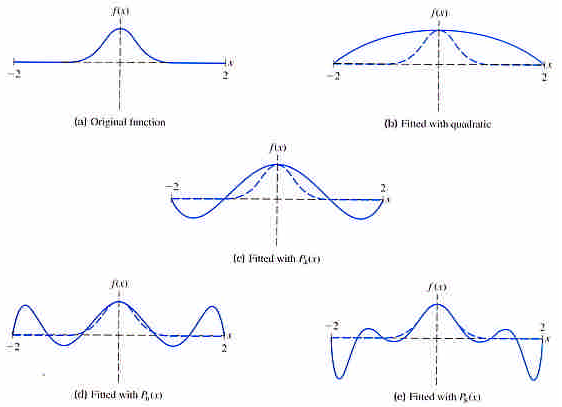
\includegraphics[width=\textwidth]{poly-int2.png}
\end{figure}
\end{columns}

\end{frame}
%---------------------
\begin{frame}
\frametitle{插值三次样条(Cubic Spline)}

\begin{figure}
\center
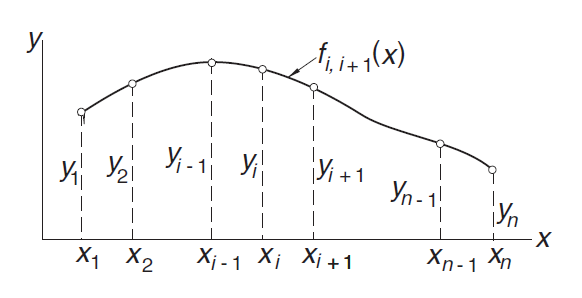
\includegraphics[width=0.5\textwidth]{cubic-int.png}
\end{figure}

设$[a,b]$上的一个划分$\triangle:a=x_0<x_1<\cdots<x_n=b$,如果
\begin{gather*}
	S|_{[x_i,x_{i+1}]}\in P_3 \\
	S(x) \in C^2[a,b]
\end{gather*}
则称$S(x)$为$[a,b]$上的三次样条函数。

如果$S(x_i)=y_i,i=0,1,...,n$,则称$S(x)$为插值三次样条函数。
\end{frame}
%---------------------
\begin{frame}
\frametitle{插值三次样条}

为构造插值三次样条曲线$S(x)$,需知道节点处的一阶或二阶导数,使得
\begin{gather*}
	S(x_i)=y_i \\
	S^{'}(x_i)=y_i^{'}=m_i \quad \text{or}\quad S^{''}(x_i)=y_i^{''}=M_i
\end{gather*}
当端点二阶导数已知时,利用插值得二阶导函数:
\begin{align*}
	S^{''}(x)&=M_{i-1}\frac{x_i-x}{h_i}+M_i\frac{x-x_{i-1}}{h_i} \\
	h_i &= x_i-x_{i-1}
\end{align*}
\end{frame}
%---------------------

\begin{frame}
\frametitle{插值三次样条}
\begin{itemize}
\item
积分后插值端点可得到三弯矩方程:
$S(x)=M_{i-1}\frac{(x_i-x)^3}{6h_i}+M_i\frac{(x-x_{i-1})^3}{6h_i}+(\frac{y_{i-1}}{h_i}-\frac{h_iM_{i-1}}{6})(x_i-x)+(\frac{y_{i}}{h_i}-\frac{h_iM_{i}}{6})(x-x_{i-1})\quad x \in [x_{i-1},x_i]$ 

\item
根据$S^{'}(x_{i}^{-})=S^{'}(x_{i}^{+})$即$s^{'}_i(x_{i})=s^{'}_{i+1}(x_{i})$,可以得到:
\begin{gather*}
	\textcolor{red}{\mu_iM_{i-1}+2M_i+\lambda_iM_{i+1}=3D_i \quad i=1,2,...,n-1} \\
	D_i=\frac{2}{h_i+h_{i+1}}(\frac{y_{i+1}-y_i}{h_{i+1}}-\frac{y_{i}-y_{i-1}}{h_{i}}) \\
	\lambda_i=\frac{h_{i+1}}{h_i+h_{i+1}} \quad
	\mu_i=1-\lambda_i
\end{gather*}

\item
对于$2n$个未知数$M_i$,现在只得到了$2(n-1)$个方程,还需两个边界条件才可求解
\end{itemize}
\end{frame}
%---------------------

\begin{frame}
\frametitle{插值三次样条}
如果知道边界处的一阶导数$y^{'}(a)=y^{'}_0,\: y^{'}(b)=y^{'}_n$,可以得到
\begin{align*}
	2M_0+M_1 &= \frac{6}{h_1}(\frac{y_1-y_0}{h_1}-y_0^{'})=3D_0 \\
	M_{n-1}+2M_n&=\frac{6}{h_n}(y_n^{'}-\frac{y_n-y_{n-1}}{h_n})=3D_n 
\end{align*}
关于$M_i$的方程写出矩阵形式(主对角占优的三对角矩阵,LU分解,追赶法)
\begin{equation*}
\left(
\begin{array}{*{6}c}
2 & 1 & 0 & 0 & \cdots & 0 \\
\mu_1 & 2 & \lambda_1 & 0 & \cdots & 0 \\
0 & \mu_2 & 2 & \lambda_2 & \cdots & 0 \\
\vdots & \vdots & \vdots & \ddots & \vdots & \vdots \\
0 & 0 & \cdots & \mu_{n-1} & 2 & \lambda_{n-1} \\
0 & 0 & \cdots & 0 & 1 & 2
\end{array}
\right)
\cdot
\left(
\begin{array}{c}
M_0 \\
M_1 \\
M_2 \\
\vdots \\
M_{n-1} \\
M_{n}
\end{array}
\right)
=3\left(
\begin{array}{c}
D_0 \\
D_1 \\
D_2 \\
\vdots \\
D_{n-1} \\
D_{n}
\end{array}
\right)
\end{equation*}
\end{frame}
%---------------------


\begin{frame}
\frametitle{曲线拟合(curve fitting)}
\begin{itemize}
\item
如果数据由实验所得,难免会有测量误差,此时没必要用插值来预测数据,拟合即可以很好的给出数据点的分布趋势。

\item 
数学描述:已知一组数据点$(x_i,y_i),i=1,2,...,n$,$x_i$互不相同。寻求一个函数(曲线) $y = f (x;a_1,...,a_m)$,使$f(x)$在某种准则下与所有数据点最为接近,即曲线拟合得最好。

\item
$f(x;a_1,...,a_m)$往往是根据经验事先确定,然后调整参数来达到较好的拟合效果。

\end{itemize}

\end{frame}
%---------------------

\begin{frame}
\frametitle{曲线拟合}
\begin{itemize}
\item
什么样的曲线拟合才是最好的拟合?

\item 
最小化误差函数:
\begin{equation*}
	S(a_1,a_2,...,a_m)=\sum_{i=1}^{n}|y_i-f(x_i)|^2 \quad m < n
\end{equation*}
对每个$a_j$,由函数的极值定理可知,$S(a_1,a_2,...,a_m)$达到最小时,满足:
\begin{equation*}
	\frac{\partial S}{\partial a_k}=0, \quad k=1,2,...,m
\end{equation*}

\item 上述即为最小二乘法(Least squares)
\end{itemize}

\end{frame}
%---------------------

\begin{frame}
\frametitle{线性回归(Linear regression)}
\begin{itemize}
\item
拟合函数为线性函数$f(x;a,b)=a+bx$

\item
误差函数相应为:$S(a,b)=\sum_{i=1}^{n}(y_i-a-bx_i)^2$

\item
$a,b$的求解方程为:
\begin{align*}
	\frac{\partial S}{\partial a}&=\sum_{i=1}^{n}-2(y_i-a-bx_i) \\
	&=2(-\sum_{i=1}^{n}y_i+na+b\sum_{i=1}^{n}x_i)=0\\
	\frac{\partial S}{\partial b}&=\sum_{i=1}^{n}-2(y_i-a-bx_i)x_i\\
		&=2(-\sum_{i=1}^{n}x_iy_i+a\sum_{i=1}{n}x_i+b\sum_{i=1}^{n}x_i^2)=0
\end{align*}
\end{itemize}
\end{frame}
%---------------------

\begin{frame}
\frametitle{线性回归}
求解线性方程组,得到:
\begin{align*}
	b &= \frac{\sum x_iy_i-n\bar{x}\bar{y}}{\sum x_i^2-n\bar{x}^2} 
	  = \frac{\sum y_i(x_i-\bar{x})}{\sum x_i(x_i-\bar{x})} \\
	a &= \bar{y}-\bar{x}b 
    	  = \frac{\bar{y}\sum x_i^2-\bar{x}\sum x_i y_i}{\sum x_i^2-n\bar{x}^2} \\
	\bar{x} &= \frac{\sum x_i}{n} \quad
	\bar{y} = \frac{\sum y_i}{n}
\end{align*}
\end{frame}
%---------------------


\begin{frame}
\frametitle{多项式拟合}
\begin{itemize}
\item
拟合函数为多项式函数$f(x)=\sum_{i=0}^{m}a_ix^i$

\item
误差函数相应为:$S=\sum_{i=1}^{n}(y_i-\sum_{i=0}^{m}a_ix^i)^2$

\item
系数求解方程为:
\begin{equation*}
\frac{\partial S}{\partial a_j}=-2\sum_{i=1}^{n}(y_i-\sum_{k=0}^{m}a_kx_k)x^j=0 \quad j = 0,1,...,m 
\end{equation*}

\end{itemize}


\end{frame}
%---------------------


\begin{frame}
\frametitle{多项式拟合}
记
\begin{align*}
A&=\left[
\begin{array}{*{5}c}
n & \sum x_i & \sum x_i^2 & \cdots & \sum x_i^m \\
\sum x_i & \sum x_i^2 & \sum x_i^3 & \cdots & \sum x_i^{m+1} \\
\sum x_i^2 & \sum x_i^3 & \sum x_i^4 & \cdots & \sum x_i^{m+2} \\
\vdots & \vdots & \vdots & \ddots & \vdots \\
\sum x_i^m & \sum x_i^{m+1} & \sum x_i^{m+2} & \cdots & \sum x_i^{2m} 
\end{array}
\right] \\
X &=
\left[
\begin{array}{*{5}c}
a_0 & a_1 & a_2 & \cdots & a_m
\end{array} 
\right]^T\\
B &=
\left[
\begin{array}{*{5}c}
\sum y_i &
\sum x_iy_i &
\sum x_i^2y_i &
\cdots &
\sum x_i^my_i
\end{array}
\right]^T
\end{align*}

解方程组即为:
\begin{equation*}
	AX=B \Rightarrow X=A^{-1}B
\end{equation*}

\end{frame}
















\end{document}


